% Options for packages loaded elsewhere
\PassOptionsToPackage{unicode}{hyperref}
\PassOptionsToPackage{hyphens}{url}
%
\documentclass[
  french,
  ignorenonframetext,
]{beamer}
\usepackage{pgfpages}
\setbeamertemplate{caption}[numbered]
\setbeamertemplate{caption label separator}{: }
\setbeamercolor{caption name}{fg=normal text.fg}
\beamertemplatenavigationsymbolsempty
% Prevent slide breaks in the middle of a paragraph
\widowpenalties 1 10000
\raggedbottom
\setbeamertemplate{part page}{
  \centering
  \begin{beamercolorbox}[sep=16pt,center]{part title}
    \usebeamerfont{part title}\insertpart\par
  \end{beamercolorbox}
}
\setbeamertemplate{section page}{
  \centering
  \begin{beamercolorbox}[sep=12pt,center]{part title}
    \usebeamerfont{section title}\insertsection\par
  \end{beamercolorbox}
}
\setbeamertemplate{subsection page}{
  \centering
  \begin{beamercolorbox}[sep=8pt,center]{part title}
    \usebeamerfont{subsection title}\insertsubsection\par
  \end{beamercolorbox}
}
\AtBeginPart{
  \frame{\partpage}
}
\AtBeginSection{
  \ifbibliography
  \else
    \frame{\sectionpage}
  \fi
}
\AtBeginSubsection{
  \frame{\subsectionpage}
}
\usepackage{lmodern}
\usepackage{amssymb,amsmath}
\usepackage{ifxetex,ifluatex}
\ifnum 0\ifxetex 1\fi\ifluatex 1\fi=0 % if pdftex
  \usepackage[T1]{fontenc}
  \usepackage[utf8]{inputenc}
  \usepackage{textcomp} % provide euro and other symbols
\else % if luatex or xetex
  \usepackage{unicode-math}
  \defaultfontfeatures{Scale=MatchLowercase}
  \defaultfontfeatures[\rmfamily]{Ligatures=TeX,Scale=1}
\fi
% Use upquote if available, for straight quotes in verbatim environments
\IfFileExists{upquote.sty}{\usepackage{upquote}}{}
\IfFileExists{microtype.sty}{% use microtype if available
  \usepackage[]{microtype}
  \UseMicrotypeSet[protrusion]{basicmath} % disable protrusion for tt fonts
}{}
\makeatletter
\@ifundefined{KOMAClassName}{% if non-KOMA class
  \IfFileExists{parskip.sty}{%
    \usepackage{parskip}
  }{% else
    \setlength{\parindent}{0pt}
    \setlength{\parskip}{6pt plus 2pt minus 1pt}}
}{% if KOMA class
  \KOMAoptions{parskip=half}}
\makeatother
\usepackage{xcolor}
\IfFileExists{xurl.sty}{\usepackage{xurl}}{} % add URL line breaks if available
\IfFileExists{bookmark.sty}{\usepackage{bookmark}}{\usepackage{hyperref}}
\hypersetup{
  pdftitle={Alba Marina Málaga Sabogal},
  pdfauthor={Audition pour le poste de maître de conférences n°4730},
  pdflang={fr},
  hidelinks,
  pdfcreator={LaTeX via pandoc}}
\urlstyle{same} % disable monospaced font for URLs
\newif\ifbibliography
\usepackage{longtable,booktabs}
\usepackage{caption}
% Make caption package work with longtable
\makeatletter
\def\fnum@table{\tablename~\thetable}
\makeatother
\usepackage{graphicx}
\makeatletter
\def\maxwidth{\ifdim\Gin@nat@width>\linewidth\linewidth\else\Gin@nat@width\fi}
\def\maxheight{\ifdim\Gin@nat@height>\textheight\textheight\else\Gin@nat@height\fi}
\makeatother
% Scale images if necessary, so that they will not overflow the page
% margins by default, and it is still possible to overwrite the defaults
% using explicit options in \includegraphics[width, height, ...]{}
\setkeys{Gin}{width=\maxwidth,height=\maxheight,keepaspectratio}
% Set default figure placement to htbp
\makeatletter
\def\fps@figure{htbp}
\makeatother
\setlength{\emergencystretch}{3em} % prevent overfull lines
\providecommand{\tightlist}{%
  \setlength{\itemsep}{0pt}\setlength{\parskip}{0pt}}
\setcounter{secnumdepth}{-\maxdimen} % remove section numbering
\ifxetex
  % Load polyglossia as late as possible: uses bidi with RTL langages (e.g. Hebrew, Arabic)
  \usepackage{polyglossia}
  \setmainlanguage[]{french}
\else
  \usepackage[shorthands=off,main=french]{babel}
\fi

\title{Alba Marina Málaga Sabogal}
\author{Audition pour le poste de maître de conférences n°4730}
\date{25 mai 2020}

\begin{document}
\frame{\titlepage}

\begin{frame}{Études et vie professionnelle}
\protect\hypertarget{uxe9tudes-et-vie-professionnelle}{}
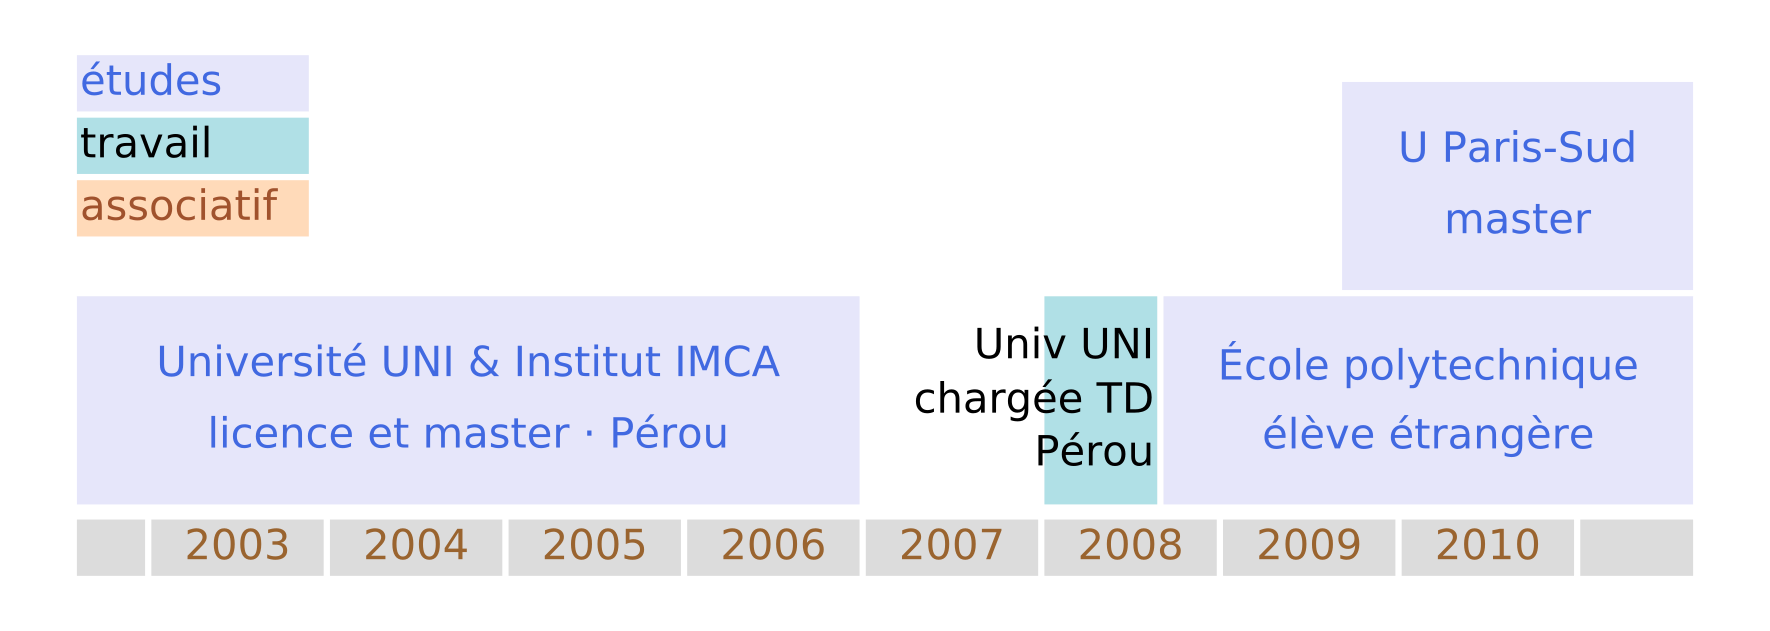
\includegraphics[width=0.9\textwidth,height=\textheight]{img/alba-timeline-etudes.png}

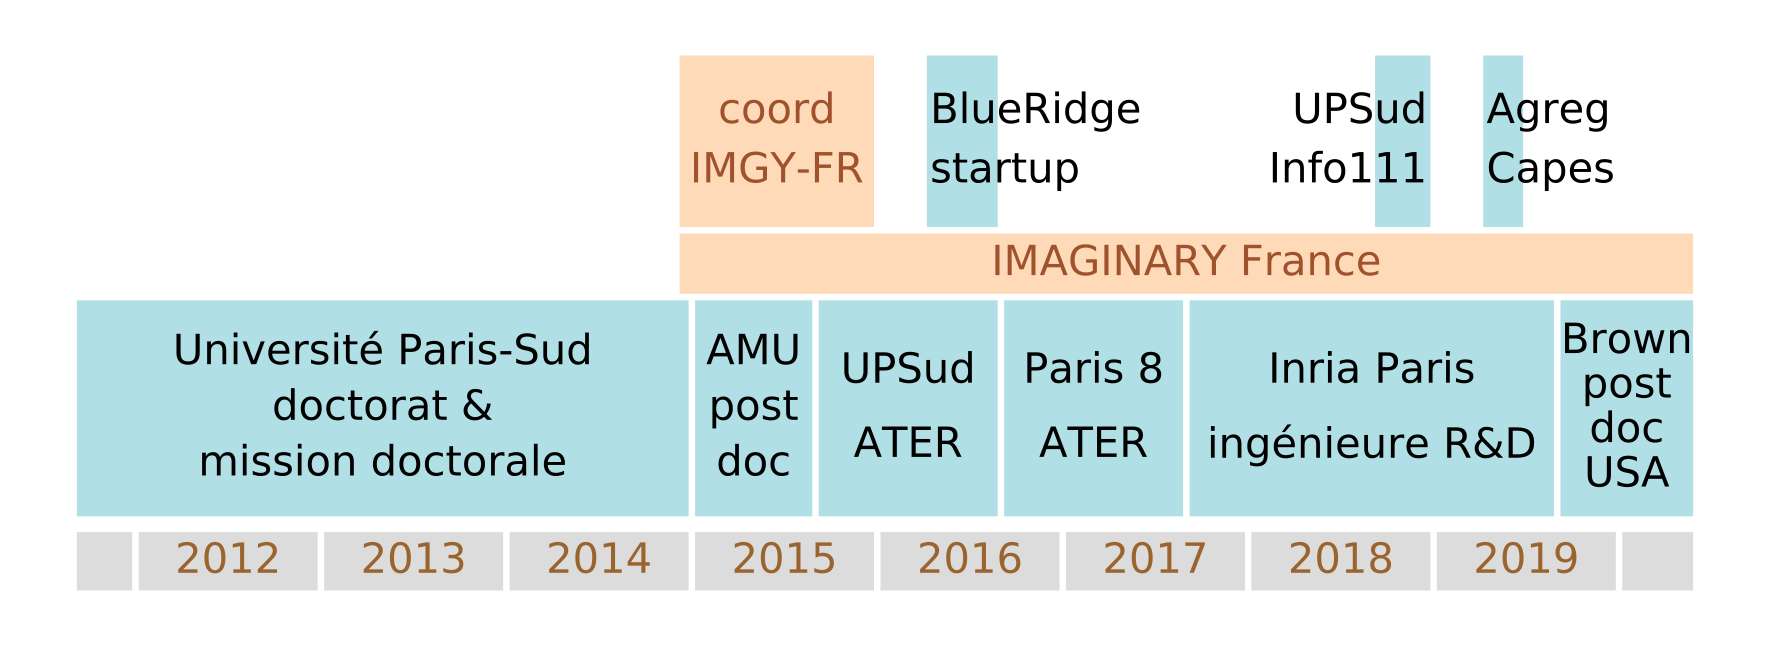
\includegraphics[width=0.9\textwidth,height=\textheight]{img/alba-timeline-viepro.png}
\end{frame}

\begin{frame}{Mes mentors au fil du temps}
\protect\hypertarget{mes-mentors-au-fil-du-temps}{}
J'ai travaillé avec:

\begin{longtable}[]{@{}lcll@{}}
\toprule
\endhead
Gilles Courtois &

\includegraphics[width=\textwidth,height=0.035\textheight]{img/logo-x.png}
& Projet sc. collectif & 2009--2010\tabularnewline
Vadim Lyubashevsky &

\includegraphics[width=0.03\textwidth,height=\textheight]{img/logo-ens.png}
& M1 info & 2011\tabularnewline
Sylvie Ruette &

\includegraphics[width=0.075\textwidth,height=\textheight]{img/logo-upsaclay.png}
& M2 math & 2011\tabularnewline
Jean-Christophe Yoccoz &

\includegraphics[width=0.075\textwidth,height=\textheight]{img/logo-cdf.jpg}
& Thèse & 2011--2014\tabularnewline
Alexander Bufetov &

\includegraphics[width=0.075\textwidth,height=\textheight]{img/logo-amu.png}
& Post-doc & 2015\tabularnewline
Richard Schwartz &

\includegraphics[width=0.075\textwidth,height=\textheight]{img/logo-brown.png}
& Post-doc & 2019--2020\tabularnewline
\bottomrule
\end{longtable}

Depuis 2015 j'ai une collaboration suivie avec Serge Troubetzkoy sur la
dynamique de surfaces de translation de mesure infinie.
\end{frame}

\begin{frame}{Les systèmes dynamiques}
\protect\hypertarget{les-systuxe8mes-dynamiques}{}
\begin{itemize}
\tightlist
\item
  Évolution déterministe à court terme, connue
\item
  Questions concernant l'évolution à long terme
\end{itemize}

\begin{block}{Exemple: les rotations du cercle}
\protect\hypertarget{exemple-les-rotations-du-cercle}{}
Vue de plusieurs itérations.

\begin{figure}
\centering
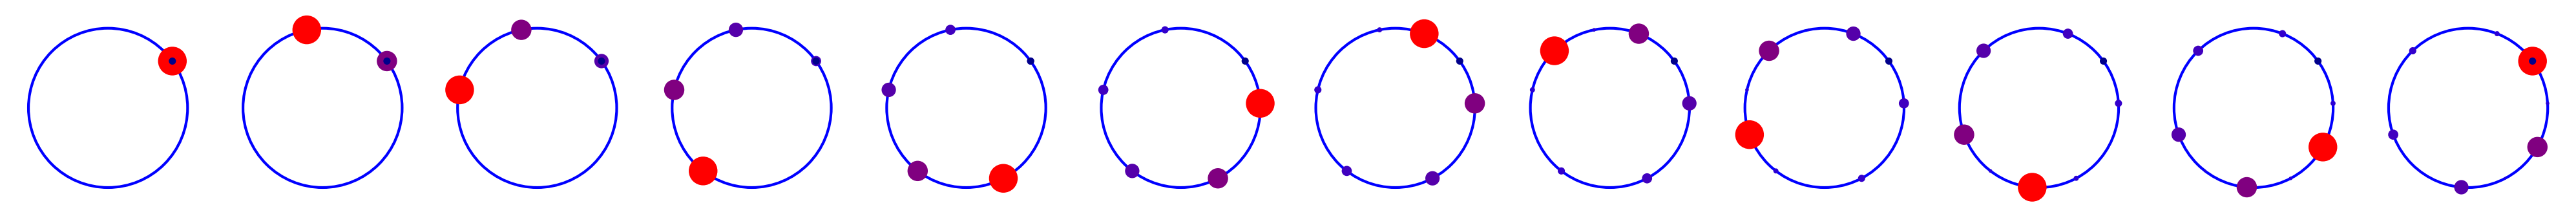
\includegraphics[width=1\textwidth,height=\textheight]{img/iteres.png}
\caption{Trajectoire d'un point par une rotation de \(\frac{2}{11}\) de
tour}
\end{figure}

\textbf{Thm} (Poincaré) Une rotation du cercle est périodique si et
seulement si elle est rationnelle. Sinon, elle est ergodique.
\end{block}
\end{frame}

\begin{frame}{Exemple: les billards}
\protect\hypertarget{exemple-les-billards}{}
\centering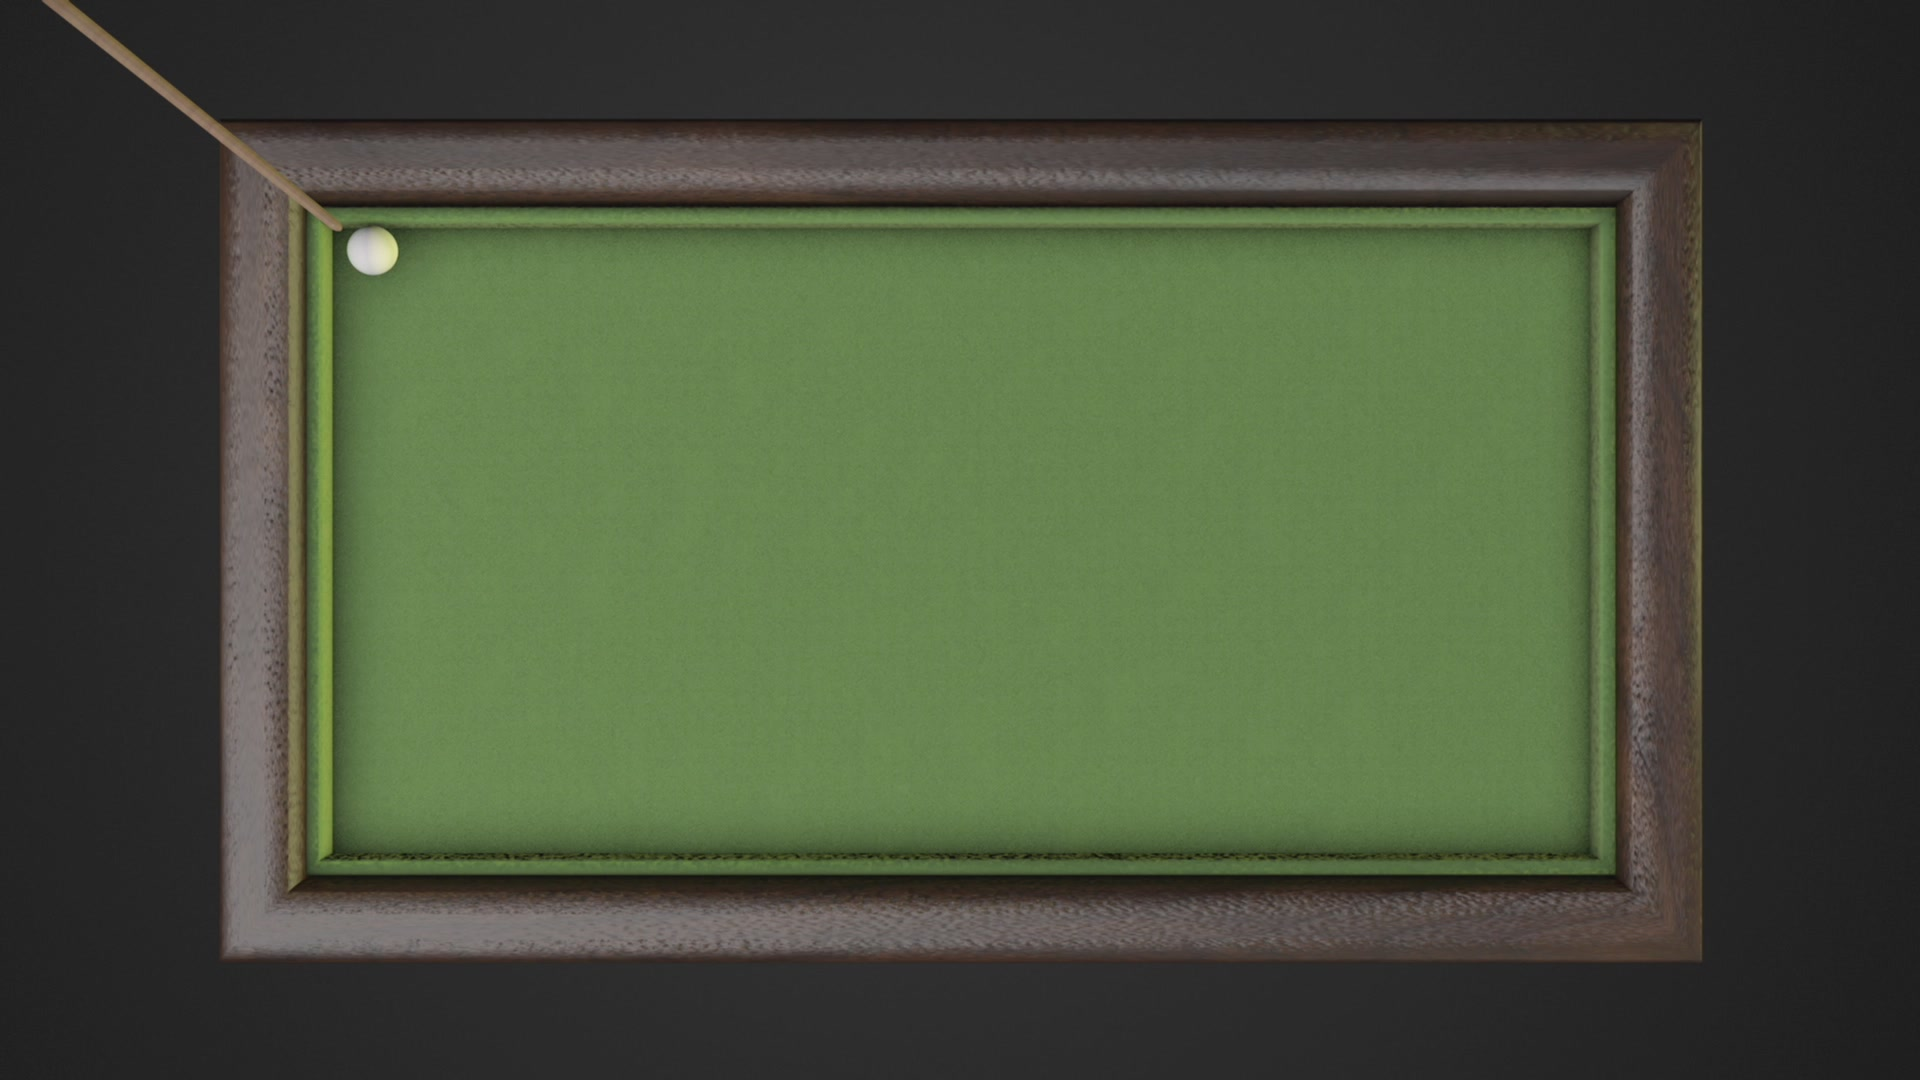
\includegraphics[width=1\textwidth,height=\textheight]{img/ball-rolling-on-a-billiard-table-0001.jpg}

\par
\end{frame}

\begin{frame}{Le dépliage des billards}
\protect\hypertarget{le-duxe9pliage-des-billards}{}
\centering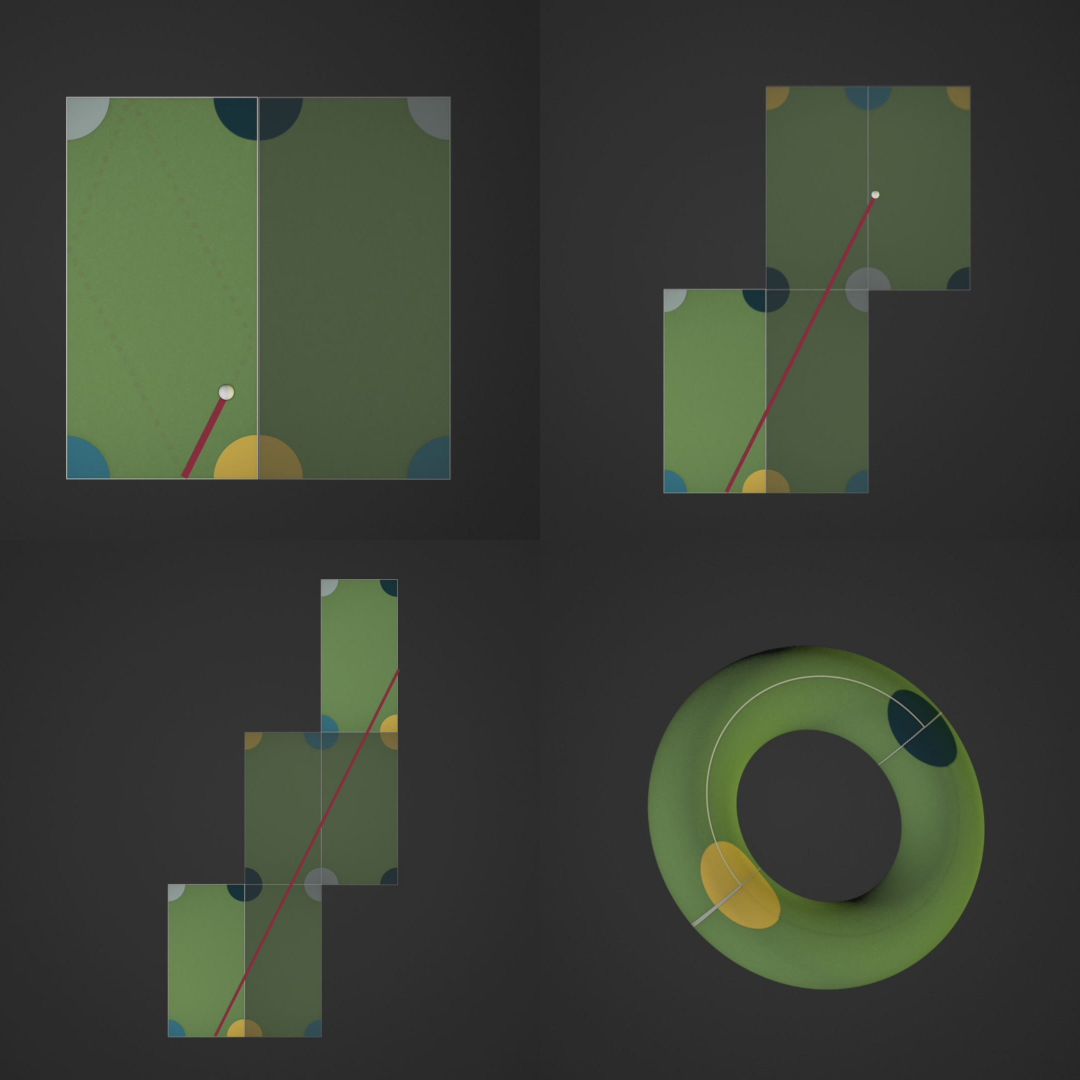
\includegraphics[width=0.75\textwidth,height=\textheight]{img/unfold-in-four-images.png}

\par
\end{frame}

\begin{frame}{Surfaces de translation et billards «infinis»}
\protect\hypertarget{surfaces-de-translation-et-billards-infinis}{}
\centering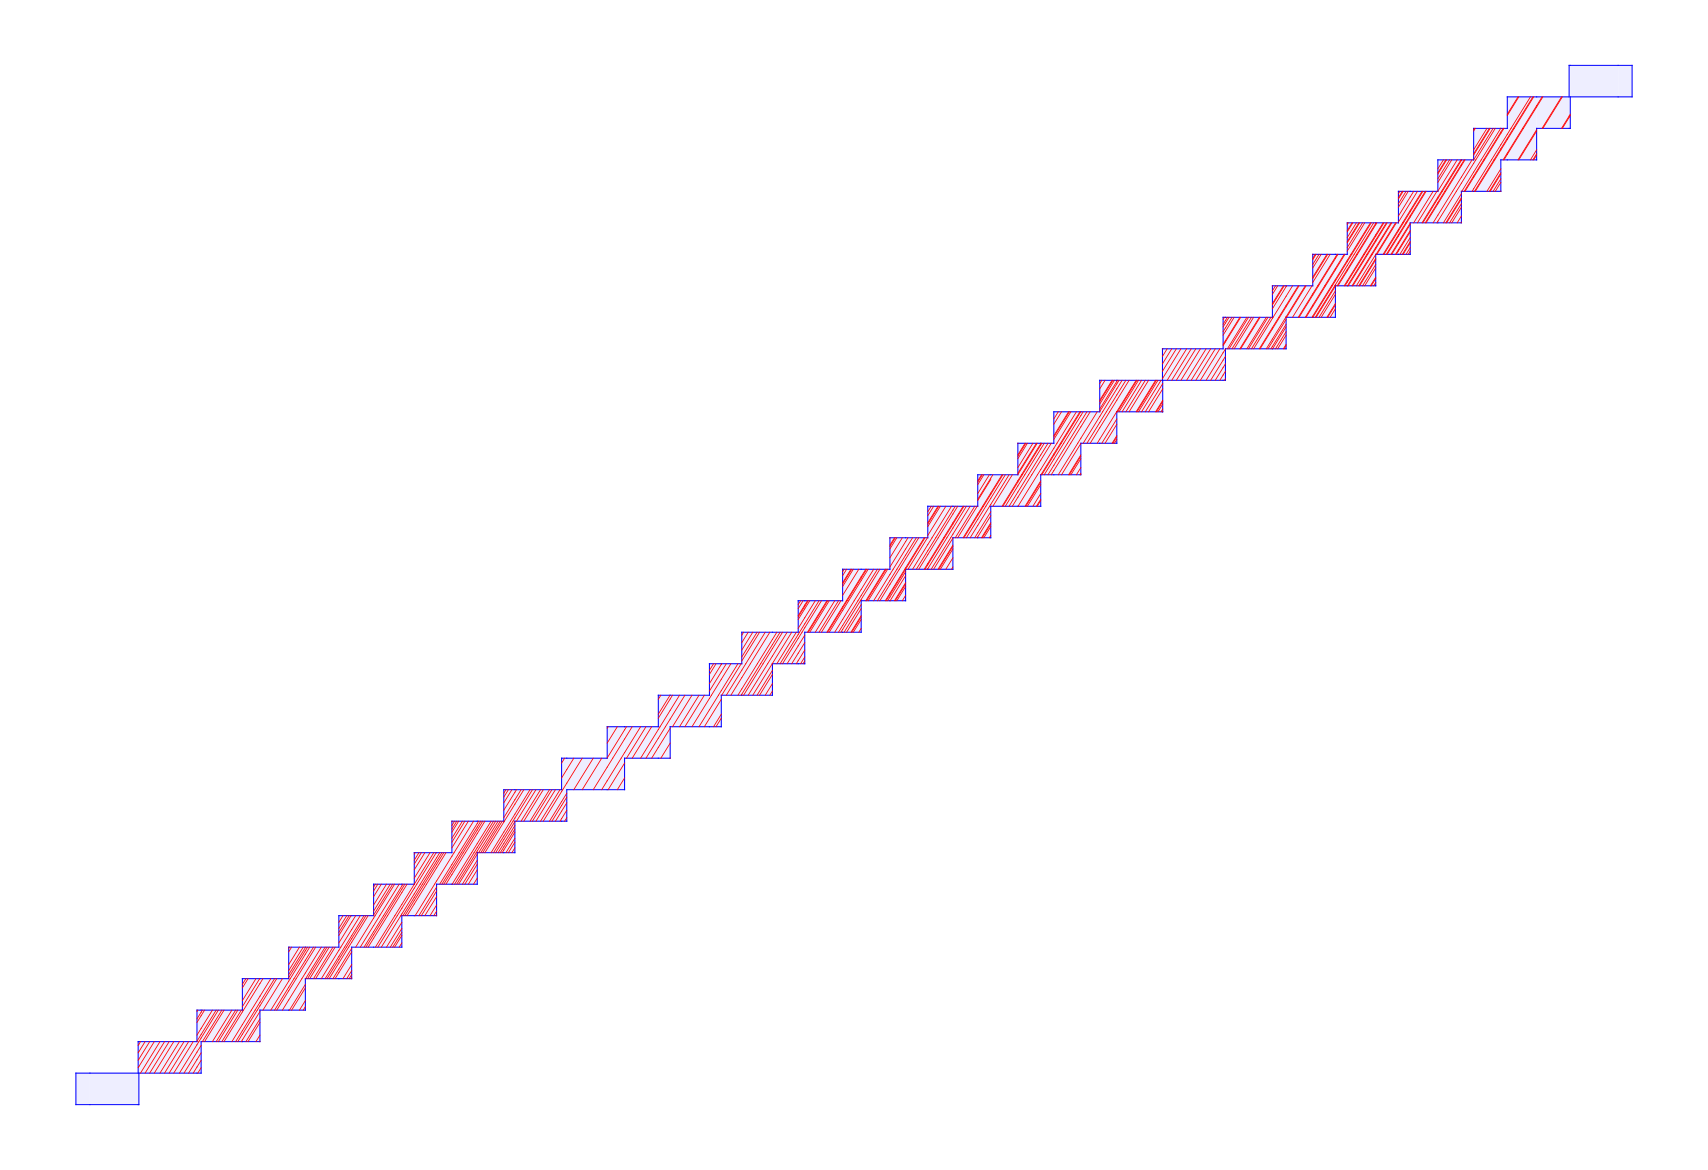
\includegraphics[width=\textwidth,height=4.6875in]{img/escalier-recollement-variable.png}

\par

\centering Escalier à recollement variable

\par
\end{frame}

\begin{frame}{Surfaces de translation et billards «infinis»}
\protect\hypertarget{surfaces-de-translation-et-billards-infinis-1}{}
\centering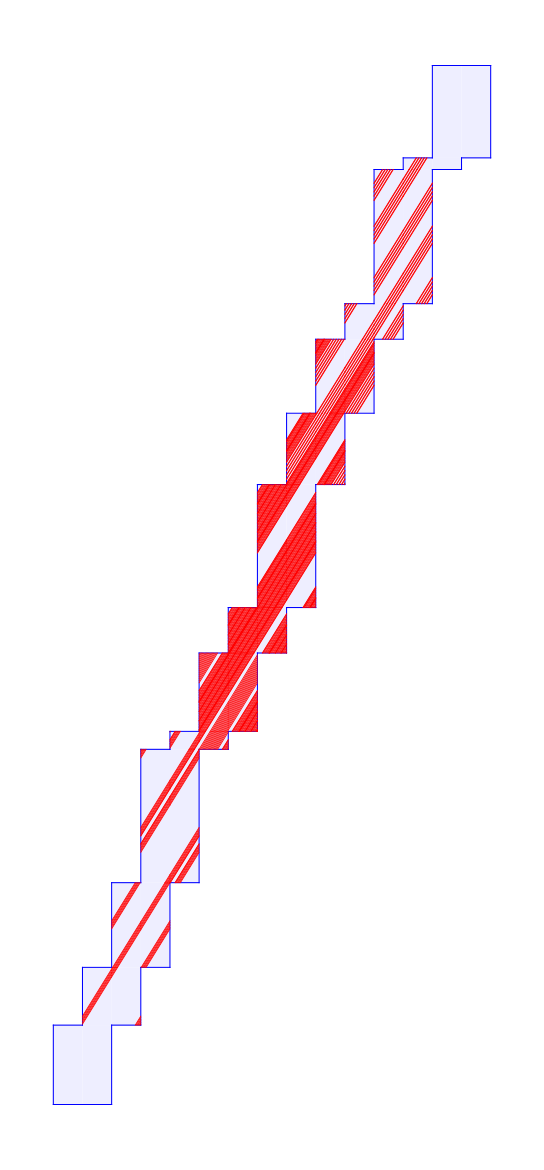
\includegraphics[width=\textwidth,height=2.91667in]{img/escalier-hauteur-variable-sage.png}

\par

\centering Escalier à hauteur variable

\par
\end{frame}

\begin{frame}{Surfaces de translation et billards «infinis»}
\protect\hypertarget{surfaces-de-translation-et-billards-infinis-2}{}
\centering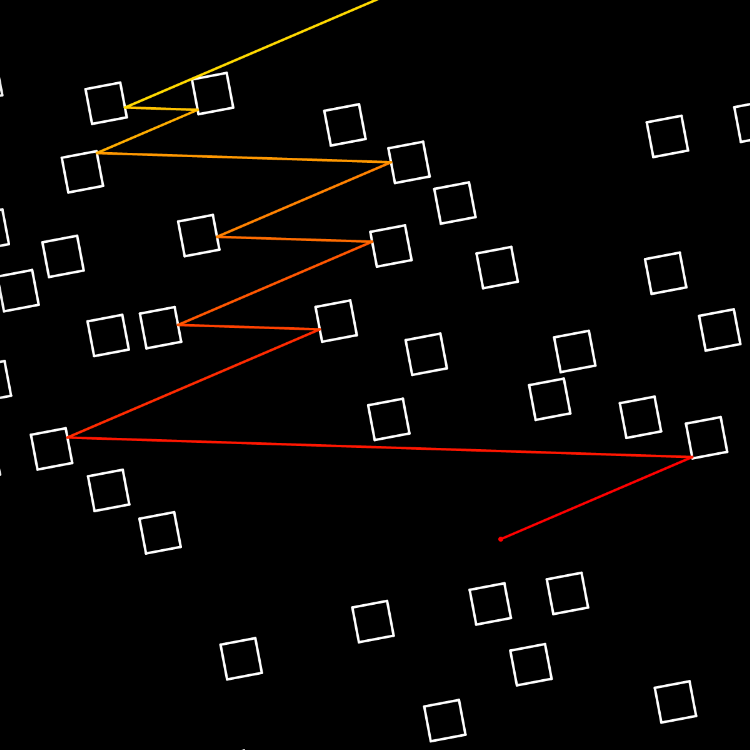
\includegraphics[width=0.6\textwidth,height=\textheight]{img/wind-tree.png}

\par

\centering Wind-tree

\par
\end{frame}

\begin{frame}{Ma thèse}
\protect\hypertarget{ma-thuxe8se}{}
J'ai soutenu en 2014 à Orsay une thèse de doctorat intitulée

\emph{Étude d'une famille de transformations\\
préservant la mesure de \(ℤ × 𝕋\).}

sous la direction de Jean-Christophe Yoccoz (Collège de France).

Résultats sur \(ℤ × 𝕋\) \(\longleftrightarrow\) escaliers infinis.

\textbf{Thm} (2014) Direction fixée, escalier générique:\\
dynamique conservative, minimale et ergodique.
\end{frame}

\begin{frame}{Mes travaux avec Serge Troubetzkoy}
\protect\hypertarget{mes-travaux-avec-serge-troubetzkoy}{}
Nous poussons beaucoup plus loin les thèmes de ma thèse.

\textbf{Thm} (2015) Génériquement, la dynamique du wind-tree est
minimale dans un large ensemble de directions.

\textbf{Thm} (2016) Génériquement, la dynamique du wind-tree dans
presque toute direction est ergodique.

\textbf{Thm} (2016) La dynamique d'un billard VH est faiblement
mélangeante dans un large ensemble de directions.

\textbf{Thm} (2017) Génériquement, la dynamique du wind-tree est
d'indice ergodique infini dans un large ensemble de directions.

\textbf{Thm} (2019) Génériquement, la dynamique des surfaces en escalier
est uniquement ergodique dans un large ensemble de directions.

\textbf{Thm} (2019) Génériquement, la dynamique du wind-tree est
uniquement ergodique dans un large ensemble de directions.
\end{frame}

\begin{frame}{Future recherche au sein du LAMA}
\protect\hypertarget{future-recherche-au-sein-du-lama}{}
Équipe: analyse harmonique

On y mélange analyse, probabilités, fractals, et dynamique symbolique.

Collaborations possibles: Mihalache, Liao, \ldots{}

Équipe Probabilités et statistiques: Julien Brémont, \ldots{}\\
Équipe Géométrie et courbure: Benoît Kloeckner

Découvrir: analyse multifractale, applications et interactions avec
systèmes dynamiques.

La forte présence du LAMA dans la communauté m'attire: GDR AMF, écoles à
Porquerolles, séminaires SCAM et COOL.
\end{frame}

\begin{frame}{Cours, cours intégrés, TD}
\protect\hypertarget{cours-cours-intuxe9gruxe9s-td}{}
Enseignements déjà dispensés:

\begin{itemize}
\tightlist
\item
  Équations différentielles
\item
  Mathématiques numériques avec Python
\item
  Calculus
\item
  Analyse
\item
  Calcul formel avec SageMath
\item
  Structures algébriques
\item
  Gestion de contenu avec Wordpress
\item
  Algèbre linéaire
\item
  Calcul vectoriel
\item
  Calcul intégral
\item
  Programmation orientée objet avec Java
\item
  Introduction à l'informatique avec C++
\end{itemize}
\end{frame}

\begin{frame}{Cours de mathématiques à la FSEG à Créteil}
\protect\hypertarget{cours-de-mathuxe9matiques-uxe0-la-fseg-uxe0-cruxe9teil}{}
Bases mathématiques de modélisation économique et de gestion,\\
en licence. Dans les maquettes actuelles:

\begin{longtable}[]{@{}ll@{}}
\toprule
Année & Intitulé du cours\tabularnewline
\midrule
\endhead
Parcours amenagé & Mathématiques\tabularnewline
& Statistiques descriptives I\tabularnewline
L1 & Mathématiques\tabularnewline
& Statistiques et outils informatiques I\tabularnewline
Passerelle & Outils mathématiques\tabularnewline
& Statistiques descriptives sur Excel\tabularnewline
L2 & Mathématiques\tabularnewline
& \textbf{Probabilités, estimation et tests}\tabularnewline
L3 & \textbf{Mathématiques des systèmes dynamiques}\tabularnewline
& Processus stochastiques en finance\tabularnewline
& Optimisation dynamique\tabularnewline
\bottomrule
\end{longtable}

Master: science des données, apprentissage automatique, \ldots{}
\end{frame}

\begin{frame}{Quelques idées de projets avec des étudiants en économie}
\protect\hypertarget{quelques-iduxe9es-de-projets-avec-des-uxe9tudiants-en-uxe9conomie}{}
\begin{itemize}
\tightlist
\item
  Recensements de population universels vs randomisés
\item
  Résultats Pisa et politiques éducatives des pays de l'OCDE
\item
  Répartition des revenus: outils d'analyse,\\
  vision synchronique et diachronique
\item
  Les systèmes d'imposition et leur évolution
\item
  Croissance économique: vision à court terme et long terme
\item
  Le coût de la santé
\item
  Le financement des retraites
\end{itemize}
\end{frame}

\begin{frame}{Médiation et diffusion scientifique}
\protect\hypertarget{muxe9diation-et-diffusion-scientifique}{}
\centering 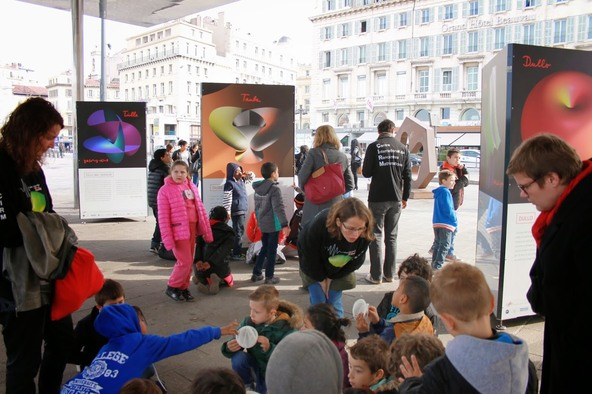
\includegraphics{img/vieux-port-alba.jpg}

\par

\centering \(\sim\) 30 expositions, forums, salons, exposés, \ldots{}

\par
\end{frame}

\begin{frame}{Médiation et diffusion scientifique}
\protect\hypertarget{muxe9diation-et-diffusion-scientifique-1}{}
\centering 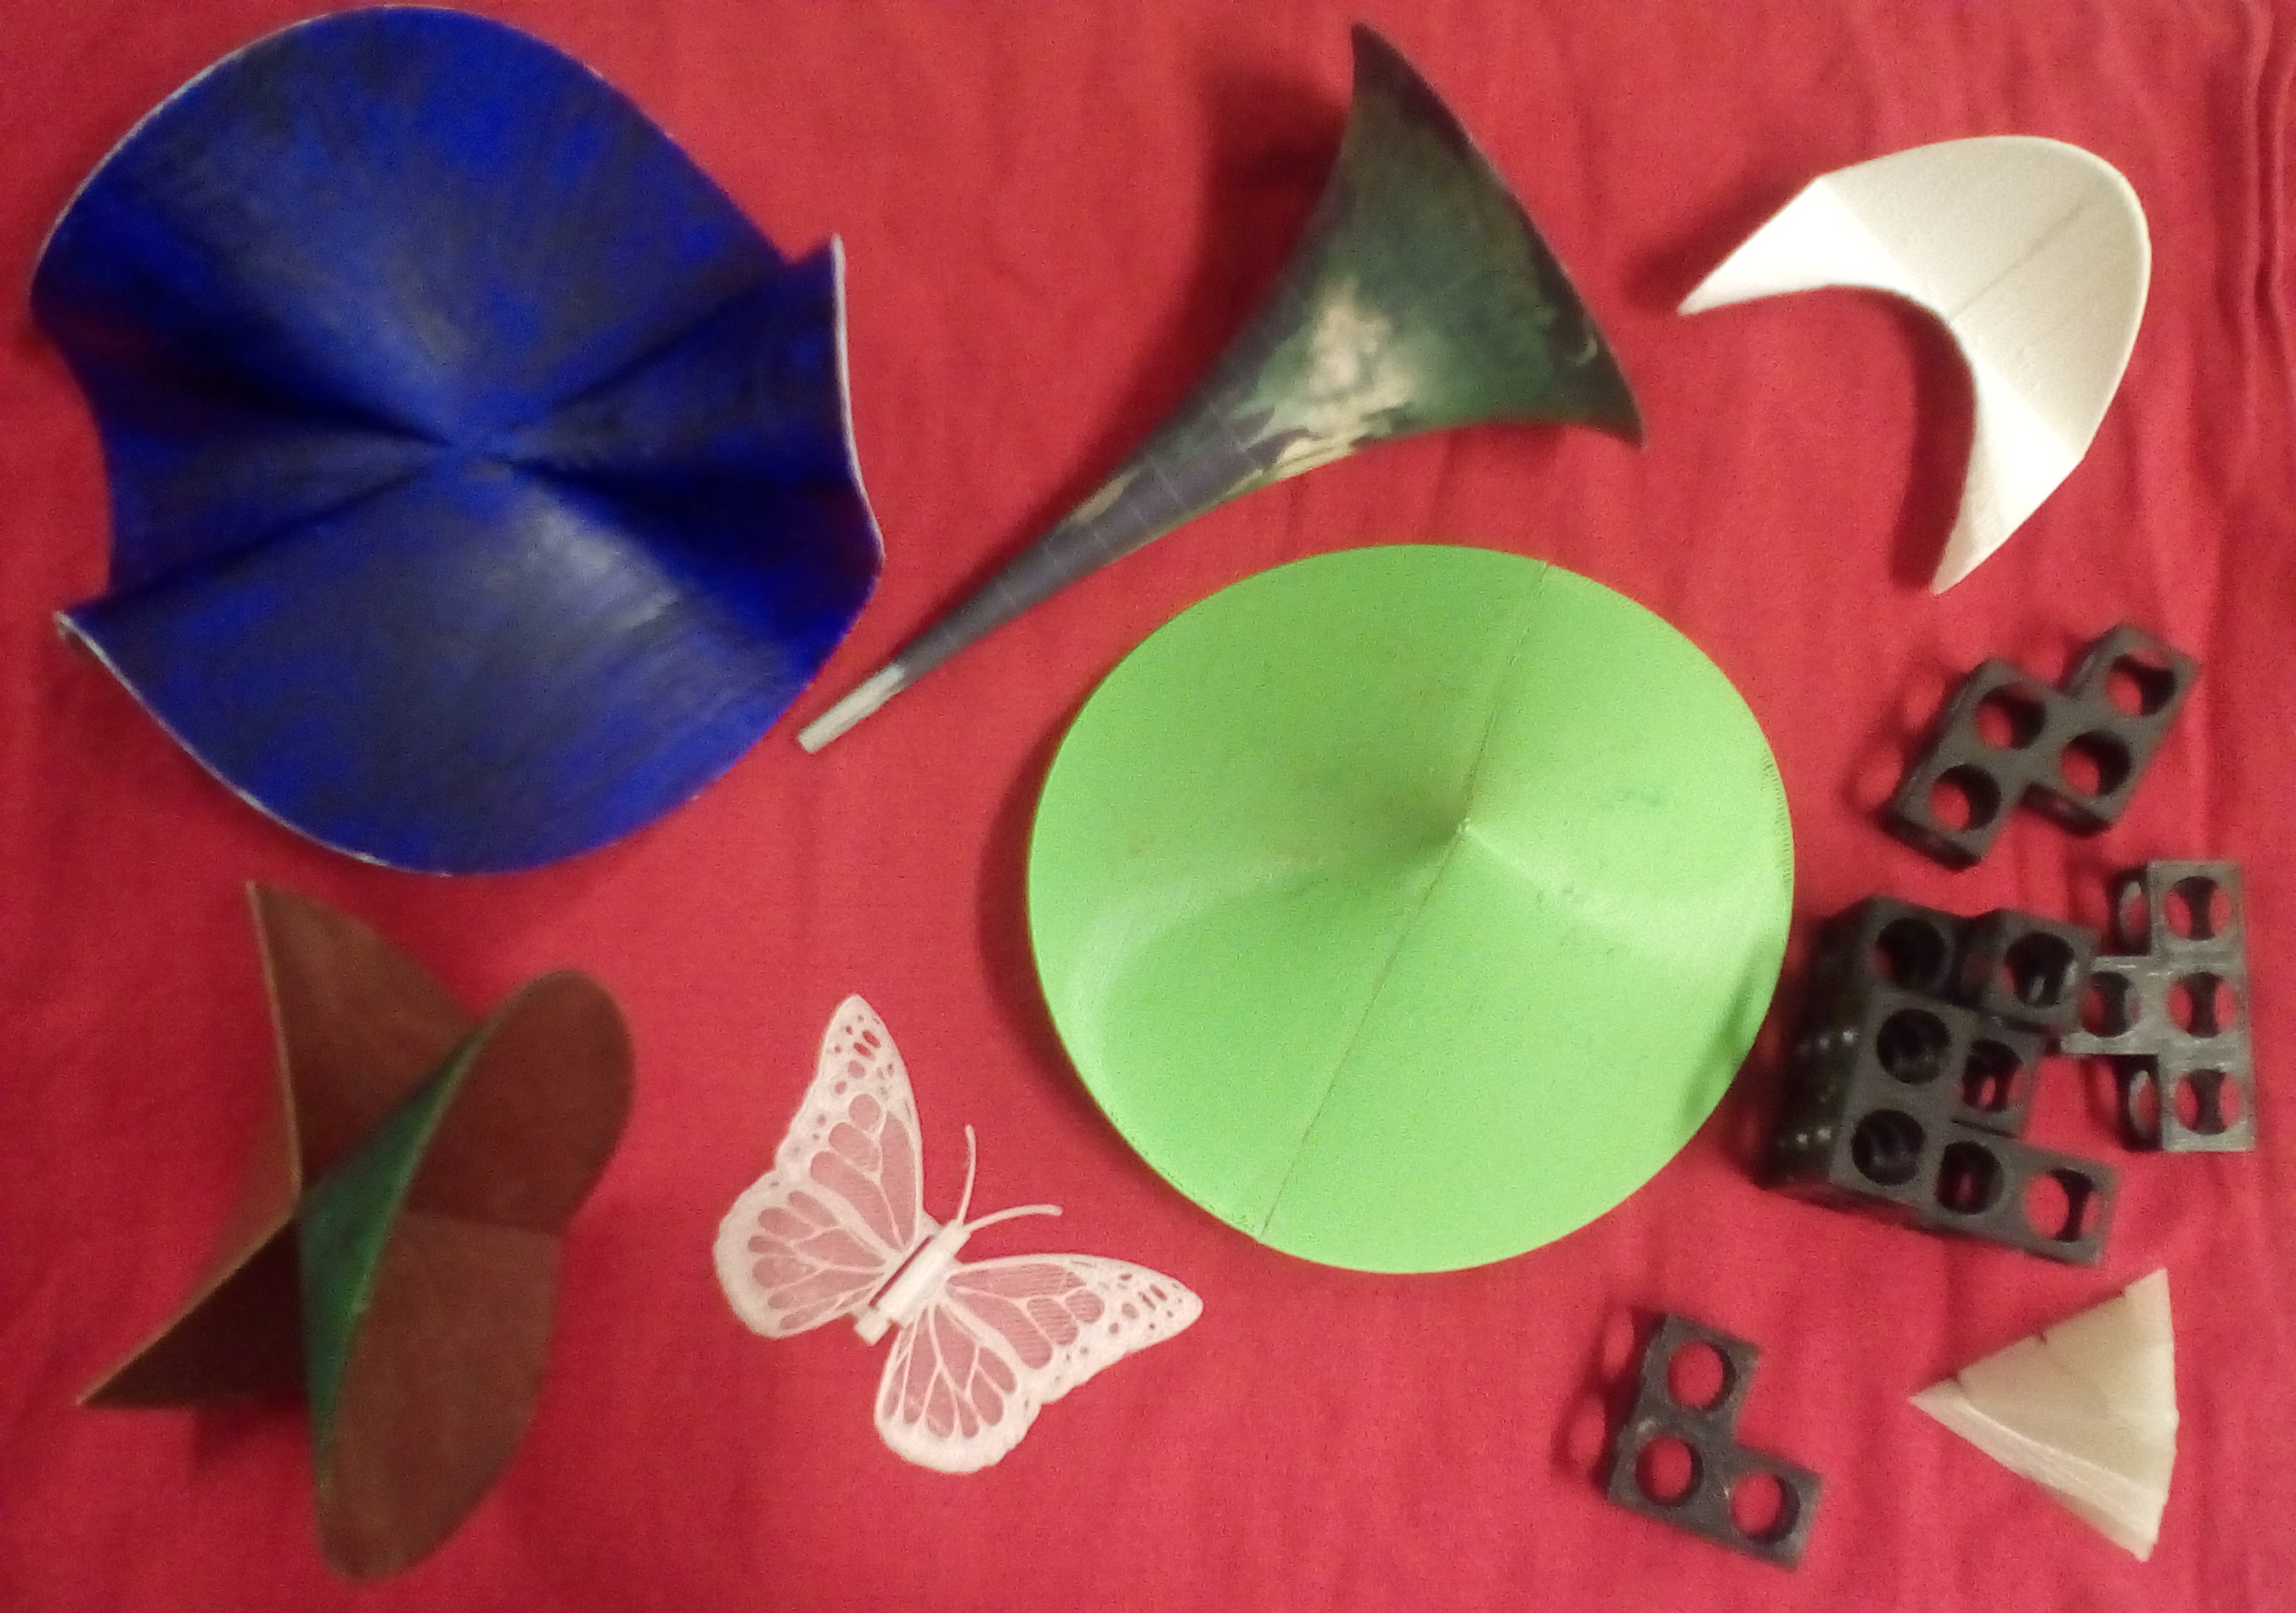
\includegraphics{img/objets-3D-sur-echarpe-rouge.png}

\par

\centering Objets mathématiques

\par
\end{frame}

\begin{frame}{Médiation et diffusion scientifique}
\protect\hypertarget{muxe9diation-et-diffusion-scientifique-2}{}
\centering 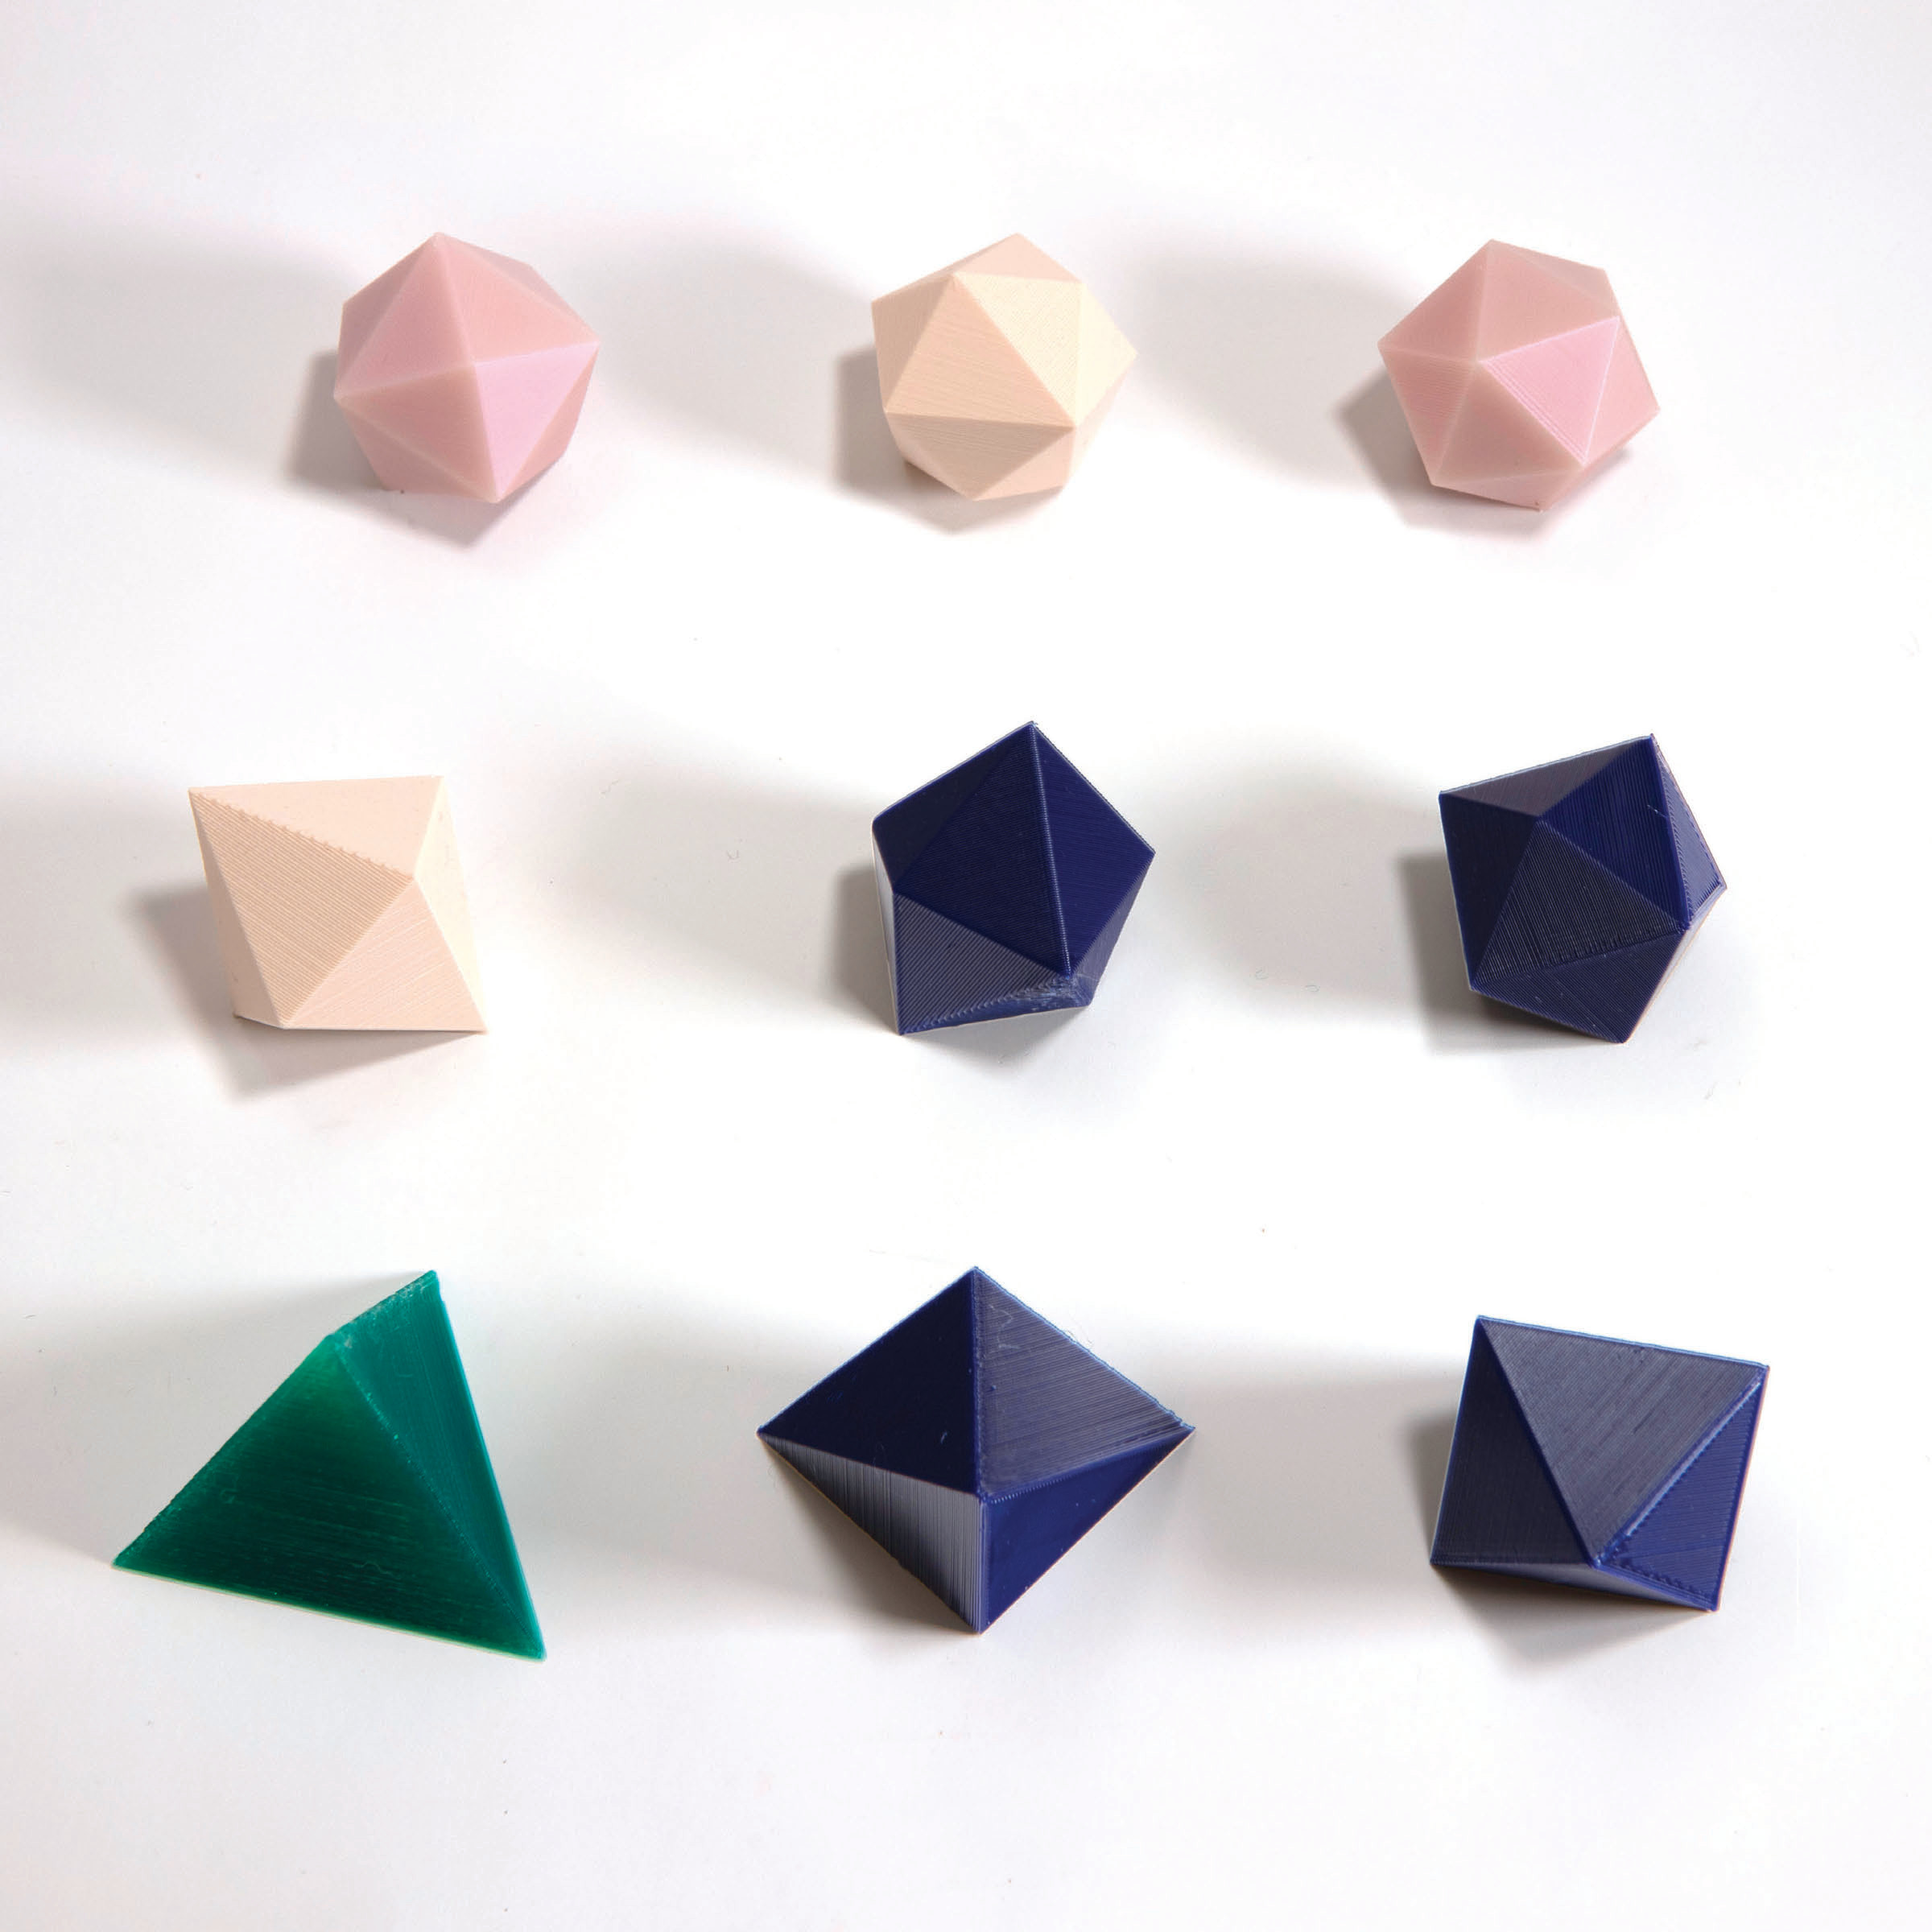
\includegraphics[width=0.6\textwidth,height=\textheight]{img/akiyama-harris.jpg}

\par

\centering Polyèdres d'Akiyama

\par
\end{frame}

\begin{frame}{Pour finir\ldots{}}
\protect\hypertarget{pour-finir}{}
\begin{longtable}[]{@{}lll@{}}
\toprule
\endhead
\begin{minipage}[t]{0.32\columnwidth}\raggedright
continuité et ouverture dans la recherche\strut
\end{minipage} & \begin{minipage}[t]{0.29\columnwidth}\raggedright
un vrai souci de l'accessibilité\strut
\end{minipage} & \begin{minipage}[t]{0.30\columnwidth}\raggedright
fibre «maker»\strut
\end{minipage}\tabularnewline
\begin{minipage}[t]{0.32\columnwidth}\raggedright
intérêt en médiation scientifique\strut
\end{minipage} & \begin{minipage}[t]{0.29\columnwidth}\raggedright
enseignement dans le respect\strut
\end{minipage} & \begin{minipage}[t]{0.30\columnwidth}\raggedright
parcours polyvalent\strut
\end{minipage}\tabularnewline
\bottomrule
\end{longtable}

J'ai à cœur de m'intégrer dans la recherche au LAMA et dans
l'enseignement à la FSEG.

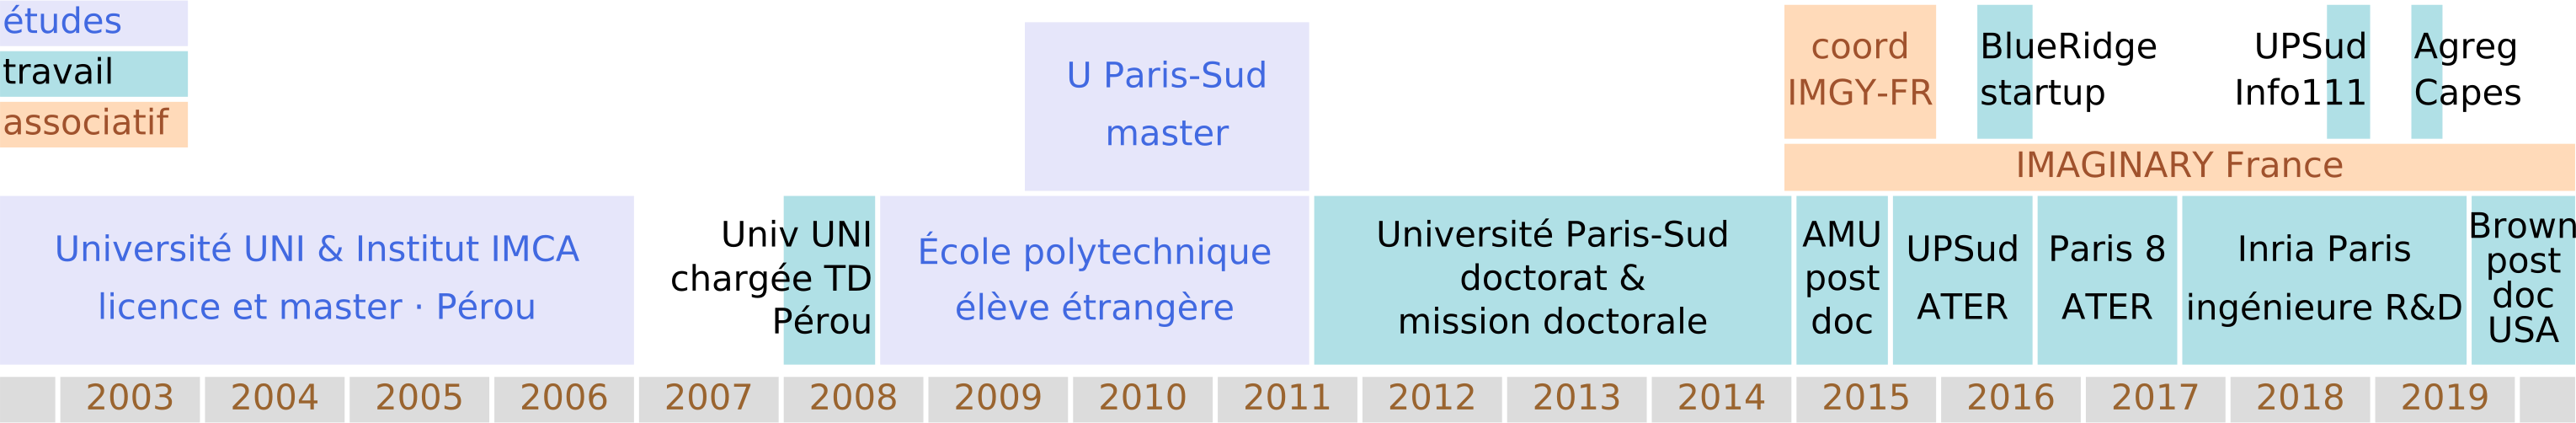
\includegraphics[width=1\textwidth,height=\textheight]{img/alba-timeline.png}
\end{frame}

\end{document}
